\documentclass{beamer}
\usetheme{Frankfurt}
%\usecolortheme{seahorse}

\title{Complex samples 1}
\subtitle{Mesocrystals, large particles and superlattices}
\author
{Walter Van Herck\inst{1}}
\institute[JCNS at MLZ] % (optional)
{
  \inst{1}%
  J\"ulich Centre for Neutron Science at MLZ
}
\date[BornAgain] % (optional)
{BornAgain School and User Meeting, 2018}
\subject{Computer Science}

\begin{document}

\frame[plain]{\titlepage}

\begin{frame}
    \frametitle{Overview}
    \tableofcontents
\end{frame}

\section{Mesocrystals}

\begin{frame}
    \frametitle{Mesocrystals}
        \begin{itemize}
            \item Mesocrystals consist of nanoparticles, ordered in a three\
                  dimensional lattice.
            \item A mesocrystal also has an outer shape.
        \end{itemize}
        \begin{figure}
            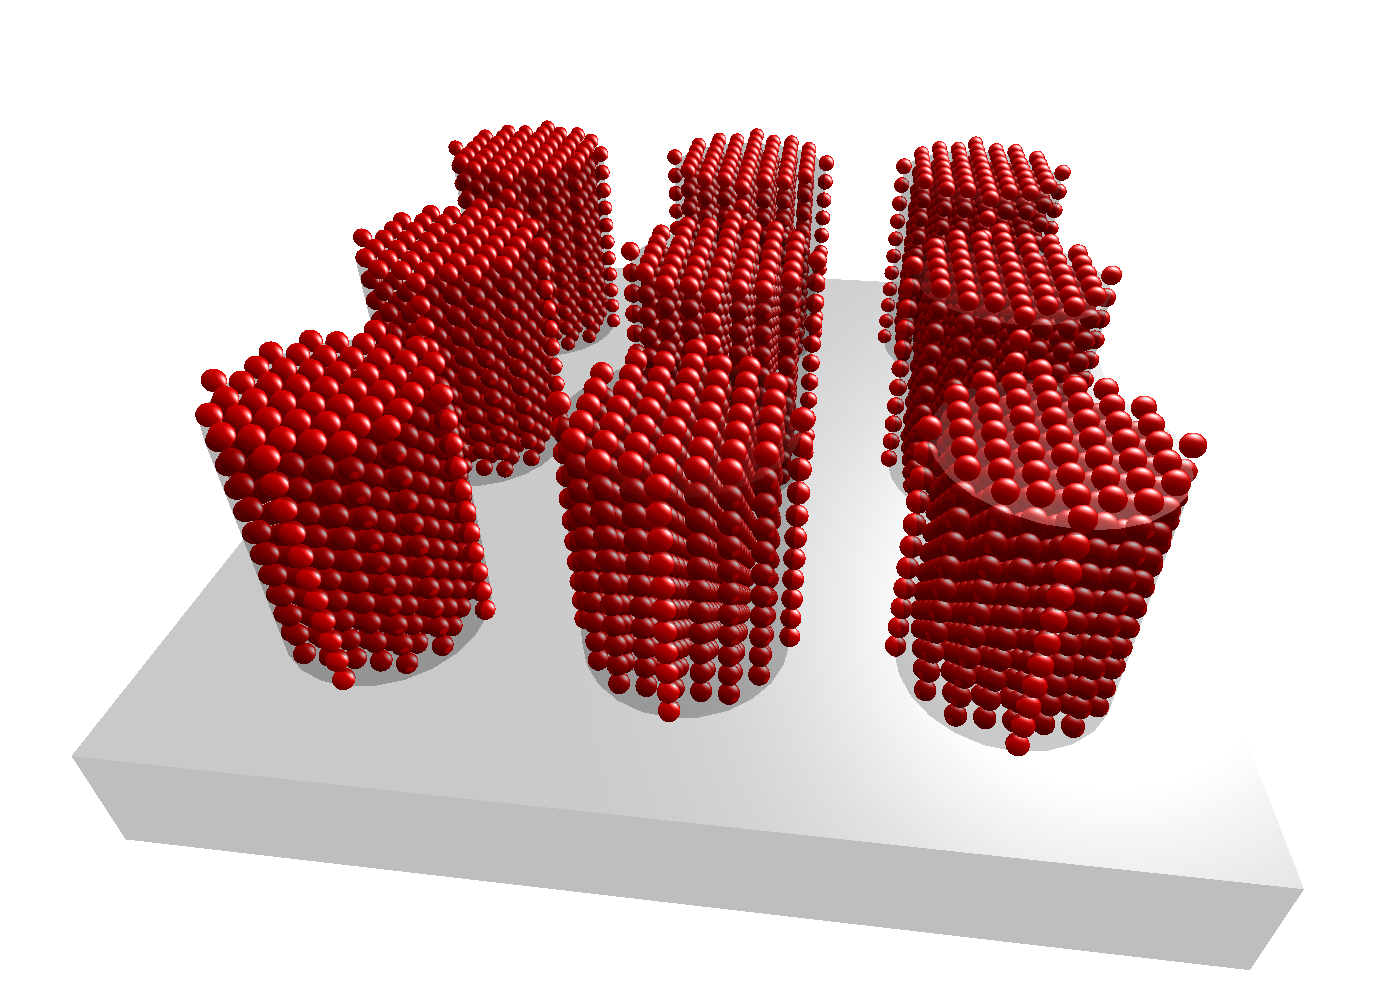
\includegraphics[width=8cm]{mesocrystal.png}
        \end{figure}
\end{frame}

\begin{frame}
    \frametitle{Mesocrystal form factor}
        \begin{itemize}
            \item The shape function of the mesocrystal is the product of its\
                  outer shape function with a 3d arrangement of nanoparticles:
                  \[ S_{meso}(\mathbf r) = S_{outer}(\mathbf r)\cdot \
                  \sum_{\mathbf{R_i}\in\Lambda} S_{nano}\left(\mathbf r - \mathbf{R_i}\right)\]
            \item The form factor then becomes a convolution:
                  \[ F_{meso}(\mathbf q) = F_{outer}(\mathbf q)\otimes \
                  \sum_{\mathbf{Q_i}\in\Lambda^*} F_{nano}(\mathbf{Q_i}) \delta\left(\mathbf q- \mathbf{Q_i}\right)\]
        \end{itemize}
\end{frame}

\section{Large particles}

\begin{frame}
    \frametitle{Large particles}
    \begin{itemize}
        \item For very large particles, the fluctuations of the scattering\
              cross section in each detector pixel cause aliasing when a\
              single sample is used.
        \item BornAgain includes the possibility of using Monte Carlo\
              integration over the pixel.
    \end{itemize}
    \begin{figure}
        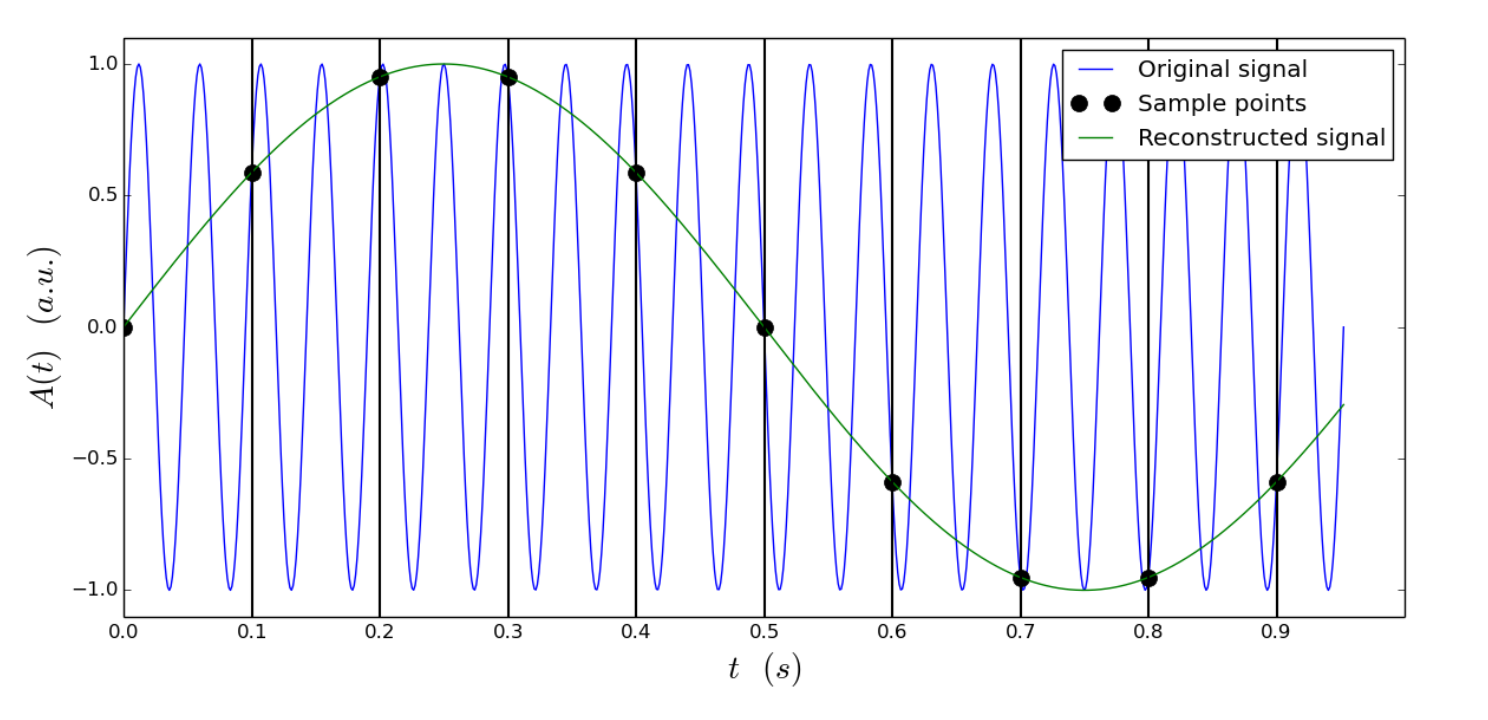
\includegraphics[width=8cm]{aliasing.png}
    \end{figure}
\end{frame}

\section{Superlattices}

\begin{frame}
    \frametitle{Superlattices}
    A superlattice consists of a finite lattice, embedded in another finite\
    lattice:
    \begin{figure}
        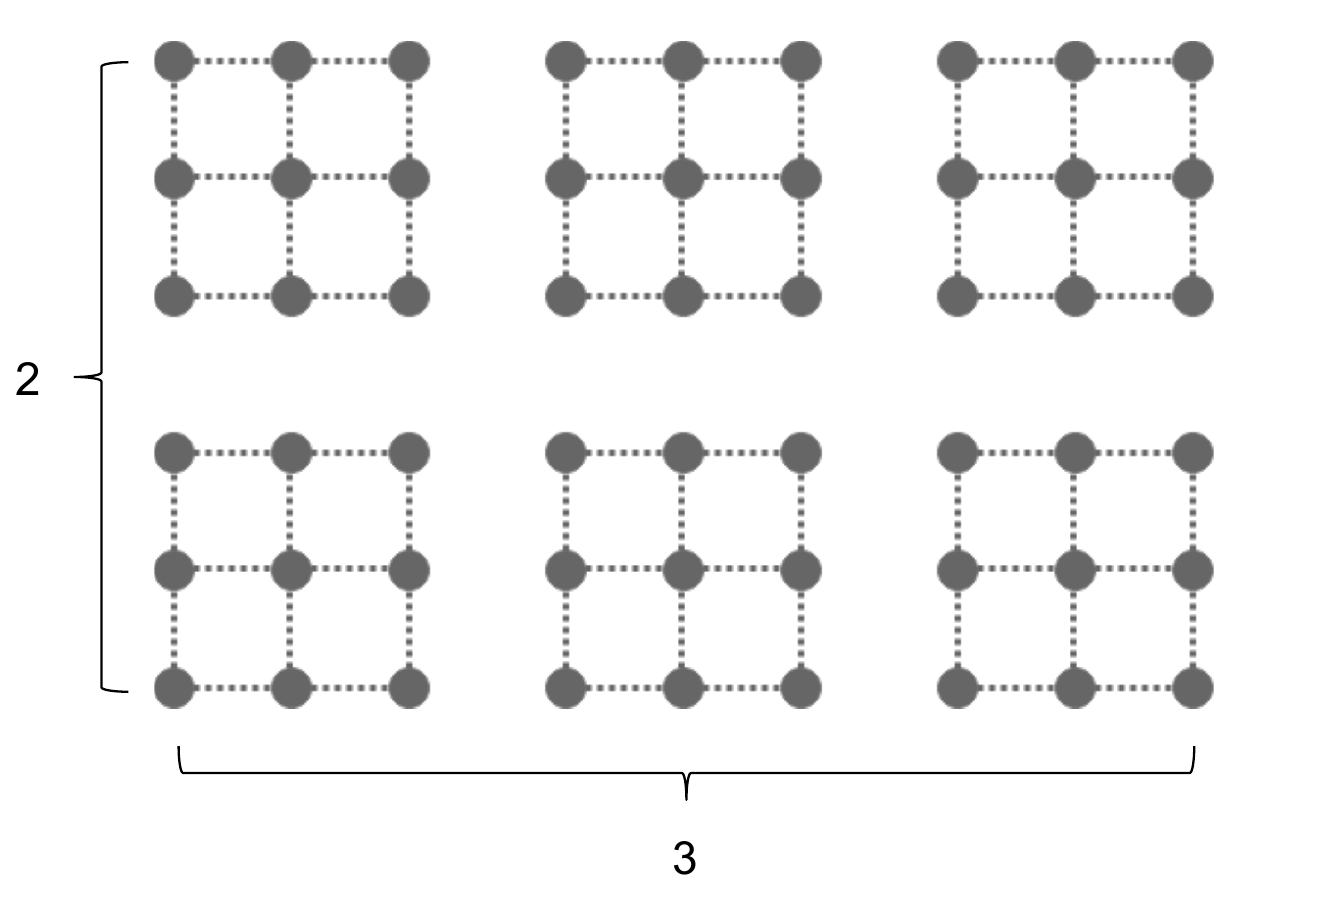
\includegraphics[width=6cm]{superlattice.png}
    \end{figure}
\end{frame}

\begin{frame}
    \frametitle{Superlattice interference function}
    The interference function can be deduced as follows:
    \begin{align}
        S(\mathbf q) &= \left| \sum_{m=1}^M \sum_{n=1}^N e^{iq(ma+nb)} \right|^2 \nonumber \\
                     &= \left| \sum_{m=1}^M e^{iqma} \sum_{n=1}^N e^{iqnb} \right|^2 \nonumber \\
                     &= \left( \frac{\sin(qMa/2)\sin(qNb/2)}{\sin(qa/2)\sin(qb/2)} \right)^2 \nonumber
    \end{align}
\end{frame}

\end{document}